\chapter{Background}
\label{cha:introQA}

This chapter will offer an overview on the relevant concepts discussed in this thesis: we will start with the definition of SAT, MaxSAT, OMT and Quantum Annealing, then we will focus on the SAT-to-Ising problem, discussing the state-of-the-art approach and why it is relevant in the field of Formal Verification.

\section{SAT and MaxSAT}
\label{sec:satmaxsat}

Computer science problems can be classified according to their computational complexity in returning a solution. Problems which complete their tasks in polynomial time with respect to their input size are known as P problems; on the other hand, NP problems are capable of simply verify if a solution satisfy the task or not in polynomial time. This thesis only addresses NP-problems and, in particular, the first discussed NP problem, SAT (Boolean satisfiability problem). \\
SAT definition is linear: given a Boolean formula as input, we try to assign the value true and false to each Boolean variable so that the resulting formula returns true. Formulas returning true for at least one assignment are called "satisfiable", otherwise they are defined "unsatisfiable". Let's discuss an example: given the following formula involving 2 Boolean variables ($x_1$ and $x_2$):

\begin{equation}
    \varphi = ( x_1 \vee x_2) \wedge (\neg x_1 \vee \neg x_2)
\end{equation}

In this case $\varphi$ is satisfiable: if we set $x_1 = T$ and $x_2 = F$, the entire formula returns true. \\
In order for a Boolean formula to be satisfiable, it is sufficient to obtain a valid assignment to solve the problem: this means that multiple solutions could be acceptable for a single formula to prove its satisfiability. Clearly the problem grows exponentially with the increase of Boolean variables: this aspect, together with the opportunity to encode other NP-complete problems into SAT, justify its popularity among computer scientists and the need to optimize it. \\
There is a vast literature focusing on SAT, discussing the theory behind this class of problems and defining algorithms and heuristic to accelerate the termination procedure. The majority of state-of-the-art solvers rely on CDCL ("conflict driven clause learning") algorithms. \\
SAT solving found real life applications in HW/SW synthesis and verification problems, cryptography and security issues and many other tasks. Currently SAT solvers are capable of managing up to $10^6$ variables and $10^7$ disjunctions for some specific case. On the other hand, more complex problems are actually out of reach despite a low number of variables to manage, for instance cryptanalysis and verification of arithmetic circuits. The search of efficiency for these tasks is the ultimate goal of our research. \\
A subclass of SAT problems is called weighted maximum satisfiability, or MaxSAT. A MaxSAT formula can be seen as optimization extension of SAT: the formula is defined as a conjunction of clauses and, for each clause, a weight (a positive real number) is assigned. Given a Boolean assignment of its variables, a score is calculated considering the weights of all satisfied clauses. This addition change the perspective of the problem: every assignment can now be considered acceptable, since some clauses can be falsified. As a consequence MaxSat defines a new task: find a Boolean assignment so that the associated score is maximum. Also in this case multiple assignment can obtain the maximum score, resulting in multiple valid assignments. \\
To better understand it, we will cover it using an example.We will consider the following Boolean formula:

\begin{equation}
    \varphi = ( x_1 \vee x_2) \wedge (\neg x_1 \vee \neg x_2) \wedge ( x_1 \vee \neg x_2) \wedge (\neg x_1 \vee x_2)
\end{equation}

Each clause has also an additional weight: first clause from left has a score of 1, each subsequent clause's weight is higher by 1 with respect to the precedent. Clearly no assignment could satisfy all clauses at the same time, but this has no interest since we are solving a MaxSAT problem. Quickly considering all possible assignments, we can state that the one guaranteeing the maximum total score is $x_1 = F$ and $x_2 = F$, satisfying respectively the clauses with weights 2, 3 and 4. No other Boolean assignment could achieve the same result, so this is the only solution to our MaxSAT problem.

\section{Satisfiability Modulo Theories}

Satisfiability Modulo Theories represents an extension to the SAT problem. The input and the final goal remain the same as SAT: this means that we have to deal with first-order logic formulas and we search for a valid assignment of variables satisfying such formulas. The main difference relies on the fact that binary boolean variables can be replaced by predicates and functions belonging to non-binary theories. Some of the most relevant theories in the Formal Verification fields are:

\begin{itemize}
    \item Linear Arithmetic over Integers, Real or both (LIRA)
    \item Bit vector arithmetic (BV)
    \item Floating-point arithmetic(FP)
    \item Uninterpreted functions (UF)
\end{itemize}

Given the non-binary nature of these theories, novel approaches have been studied and tested to efficiently evaluate the satisfiability of a given formula. At the current state, the most widely used algorithm is known as Lazy SMT solving, whose core idea will be briefly explained to the reader for a better comprehension. Given an SMT formula and a subset of theories, we produce a Boolean abstraction formula in which each non-binary predicate is replaced by a binary variable. This new formula is then fed to a CDCL SAT solver and used to search a satisfiable assignment. When a satisfiable assignment is obtained, the corresponding set of T-literals that make up the original problem are fed to specialized theory solvers. If each clause if T-consistent, then we proved the satisfibility of the original formula; otherwise, the conflict clauses causing unsatisfiability are extracted and learned by the CDCL algorithm , permitting the evaluation of new assignments. The algorithm goes on until satisfiability is proved or no more assignment can be returned, proving its unsatisfiability. \\
In order to be evaluated, the instance of a SMT problem has to be instantiated using a standard format. Regarding SMT encoding, SMT-LIB is the international initiative on top of which most SMT solvers are built. SMT-LIB does not only promote common input and output languages for SMT solvers; it also provides standard rigorous descriptions of background theories used in SMT systems and establishes benchmarks that can be used to test the solvers to highlight weaknesses and strengths. \\
The syntax of SMT-LIB-based tools is quite simple. First,we define properties of the problem and solver options (for instance determine if we want to extract unsat cores). We can also set a theory, so that efficient algorithms and heuristics are applied during execution to improve performances. After this introduction, we declare constants, variables and functions. Then assertions are expressed: they bind the values of variables, restricting the range of satisfying solutions. A simple example is provided in listing 1.1. \\
\begin{lstlisting}[style=interfaces,caption=An example of SMT-LIB encoding.]
(set-info :smt-lib-version 2.6)
(set-option :print-success false)
(set-option :produce-models true)

(declare-const x Int)
(declare-const y Int)
(declare-fun f (Int) Int)

(assert (= (f x) (f y)))
(assert (not (= x y)))

(check-sat)
(get-value (x y))
\end{lstlisting}
Among the solvers accepting SMT-LIB as input format, University of Trento and the Bruno Kessler Foundation have developed a SMT solver, called MathSAT. The code, written in C++, support all the theories mentioned above, plus other logics as Arrays arithmetic. It also supports interesting functionalities such as generation of models and proofs for satisfiable problem, extraction of unsatisfiable cores for the unsatisfiable ones and incrementality.


\section{Optimization Modulo Theories}

Optimization Modulo Theories represents an extension to the SMT framework. In addition to the already described first-order formulas involving non-binary formulas, we focus on defining one or more non-binary objective function. As a result, retrieving a satisfying assignment is not sufficient anymore: the goal is now obtaining a valid model while minimizing/maximizing the objective functions, according to our choice.\\
The language used to encode OMT problems is an extension of the SMT-LIB standards. In addition to the syntax already discussed for SMT-LIB, some commands are available to define the cost functions we desire to optimize and the direction of optimization. The structure of this command is:

\begin{equation*}
    \textbf{solve [maximize/minimize] $<$cost function$>$}
\end{equation*}

If permitted by the solver, we can also write multi-objective optimization problems. multi-objective optimization problems  require the presence of some instructions to determine the philosophy adopted to determine the goodness of a solution. Example of valid approaches are:

\begin{itemize}
    \item \textbf{Pareto Optimality}: given two different solutions and a set of $n$ cost functions $x_1...x_n$, we state that the first solution is better to the second one according to this criterion if there exists a cost function $x_i$ (where $1\leq i\leq n$) so that $x_i$ calculated on the values of the first solution dominates the value obtained using the second solution; in addition to that, for each cost function $x_i$ the first solution obtain better or equal values than the second one. When using this criterion, multiple solutions can satisfy these conditions: the set of these valid assignment is called \textbf{Pareto front}.
    \item \textbf{Lexicographic Optimality}: first we define a total order among the various cost functions, determining  a hierarchy. Given two different solutions, we will first compare the value of the first cost function on this hierarchy for both of them; if one of these solutions dominates the other it is chosen as, otherwise we will compare the value associated to the second cost function and so on until reaching the last one.
\end{itemize}

The jointly work between FBK and University of Trento gave birth to an Optimization Modulo Theories solver, \textit{OptiMathSAT}.

\section{Quantum Annealer}
\label{sec:quantum}

In order to achieve efficiency in solving the hardest tasks, one of the proposed techniques involves the exploit of quantum technologies. In the case at issue Quantum Annealers (QA) have been proved to be effective for this task. \\
Quantum annealers are specialized chips that exploit particular quantum effects (such as superposition and tunneling) to sample or minimize energy configurations. Each configuration is composed by binary variables $z_i$, called qubits, which can assume a value -1 or 1 representing their state. The energy configuration can be represented using the Ising Hamiltonian function, whose structure is the following:

\begin{equation}
    H(\textbf{\underline{z}}) = \theta + \sum_{i \in V} h_iz_i + \sum_{\langle i,j\rangle \in E} J_{ij} z_iz_j
\end{equation}

Formula 1.3 shows the parameters that influence the system's behaviour: 

\begin{itemize}
    \item $\theta$ is called \textbf{offset} and can assume any value is the Real numbers real
    \item $h_i$ are called \textbf{biases} and are defined as a real number in range $[-2,2]$
    \item $J_{ij}$ and lastly $J_{ij}$ are called \textbf{couplings} to the connected pair of qubits at index $i$ and $j$ and is a real number in range $[-1,1]$.
\end{itemize}

The search of the ground state of an Ising model is known as \textbf{quadratic unconstrained binary optimization (QUBO)} problem. \\
The entire energy configuration can be represented as a connected graph, where vertexes represent our qubits and edges represent connections between qubits. This configuration highlights how qubits' ground state is not considered independently, but their interaction with neighbour qubits alters the final energy state of our configuration. This interaction reflects the hardware architecture of a quantum annealer: qubits are built as super-conducting rings and their value defines the direction of the circulating current. Rings can be superimposed to other rings, defining the generation of couplings weights. Figure 1.1 shows the basic structure of some pairs of qubits and the idea behind of biases and couplings. \\
\begin{figure}[t]
    \begin{subfigure}{.5\textwidth}
        \centering
	    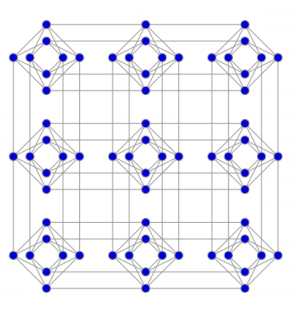
\includegraphics{QATile.PNG}
    \end{subfigure}
    \begin{subfigure}{.5\textwidth}
        \begin{center}
	    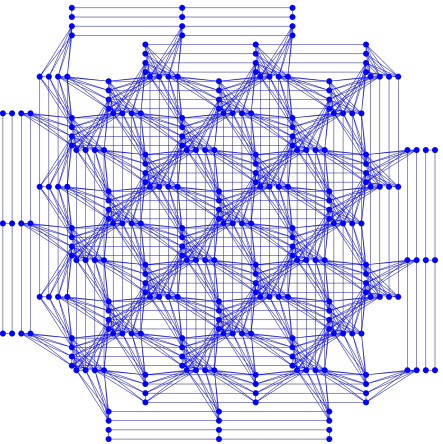
\includegraphics[width=\textwidth]{Pegas.PNG}
	    \end{center}
	\end{subfigure}
	\caption{A representation of the two architecture proposed by D-Wave, a $3*3$ tiles subgraph of Chimera (on the left) and Pegasus (on the right).}
\end{figure}
The choice of a specific quantum annealer influences the formulation of an Ising model: each annealer has a specific architecture and specific properties, constraining the formulation of a problem. In this thesis we will concentrate on annealers developed by the Canadian company D-Wave \cite{Dwave}. In the beginning, the Canadian company aimed in increasing the number of available qubits, obtaining Moore-like growth as shown in figure xx. In a second phase, the company put its effort in defining novel structures with better connections and fewer wated qubits. Currently D-Wave has already developed and produced a first quantum system, known as \textbf{Chimera}. The basic features of this architecture are:

\begin{itemize}
    \item The basic unit is the tile, which contains 8 qubits.
    \item Qubits of a cell unit are grouped into two groups (the horizontal and vertical qubits): qubits belonging to the same group are connected to qubits of the opposite group thanks to couplings.
    \item Unit cells are tiled vertically and horizontally with adjacent qubits connected, creating a 16 $\times$ 16 lattice of qubits. The number of total qubits 
    \item From previous constraints, we can see how each qubits can be connected to a maximum of 6 other variables, resulting in the sparsity of the matrix. Qubits that are not connected to each other are managed while writing the Ising formulation setting the coupling value as 0.
\end{itemize}

In addition to this structure, D-Wave is already studying new architectures overcoming the sparsity of the graph and the absence of cliques; in 2019 the company proposed a new architecture called \textbf{Pegasus}. The properties of this system are:

\begin{itemize}
    \item The number of qubits is $24*N*(N-1)$, where $N$ is an integer number selectable by the users according to their needs.
    \item The architecture is less modular than Chimera and, in particular, it is not structured in 8-qubit tiles.
    \item Pegasus graph is less sparse than Chimera, presenting an higher number of interleavings among qubits (exactly 15 couplers for a single qubit).
    \item The increasing number of couplers have given the opportunity to obtain huge progress with respect to the old model. In particular, Pegasus provides 3 and 4-cliques and qubit duplication.
\end{itemize}

Figure 1.2 shows the graphs representing both Chimera and Pegasus topologies, rapidly displaying the main differences between the two models. 

\begin{figure}[t]
	\begin{center}
	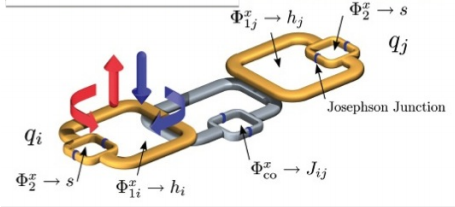
\includegraphics{QA.PNG}
	\caption{Lorem Ipsum.}
	\end{center}
\end{figure}

\section{SAT-to-Ising}
\label{sec:SATtoQUBO}

Once defined the two main concepts behind this dissertation, let's discuss the binding between them. As already stated in the previous paragraphs, SAT's main issue is the exponential growth of complexity, stopping computer scientists in investigating hard tasks involving a small number of variables. Quantum computing, on the other hand, exploit specific phenomena such as tunneling to search the minimum of an Ising problem, optimizing computational time. If we would be able to encode SAT/MaxSAT problem into an Ising Hamiltonian problem, we could exploit quantum calculus properties to verify satisfiability of out original problems, drastically reducing computational time. The task described is known as \textbf{SAT-to-QUBO}, where QUBO stands for \textit{Quadratic Uncostrained Boolean Optimization}. \\
Computer scientists use Quantum Annealers as black-box algorithms which are fed to QUBO problems, whose formulation is similar but not identical to an Ising problem:

\begin{equation}
    FORMULA
\end{equation}

As we can see qubits, biases and couplings are present in our formulation; in addition to them we consider the parameter $\theta_0$, which is called offset and falls into the range $(+\infty, -\infty)$. \\
Given a SAT problem, we are interested in finding a variable placement \textbf{x} $\rightarrow$ \textbf{z} on the quantum annealer qubits and the values of offset, biases and couplings so that:

\begin{equation}
    P_F(\underline{\textbf{x}} | \underline{\theta}) = 
    \left\{
        \begin{array}{lr}
            = 0, & if \textbf{ \underline{x}} \models F \\
            \geq g_{min}, & if \textbf{ \underline{x}} \models T
        \end{array}
    \right\}
\end{equation}

The gap $g_{min}$ is essential to manage sensitivity of the quantum annealer: the optimization will be affected by noise generated by the non-zero Kelvin temperature and , so it will be rarely the case that not satisfying assignment will get 0 as final score. Setting the gap (and trying to find the highest gap possible satisfying the problem) will help us in discriminating acceptable assignments and not acceptable ones.
For instance, a formula we can easily encode into an Ising Hamiltonian function is $\varphi = x_1 \iff x_2$. A simple penalty function would be $P_F(\underline{\textbf{x}} | \underline{\theta}) = 1 - x_1x_2$, whose gap for satisfying assignment is 2. \\
The current formulation of our problem presents some issues:

\begin{itemize}
    \item Chimera tile architecture is quite limited: the absence of clique and the sparsity of the matrix reduce the number of problem we can represent.
    \item The problem is actually overconstrained: you need to search your solution checking O($2^{|\textbf{\underline{x}}|}$) models/countermodels. You have also to deal with the degrees of freedom of its formulation caused by biases and couplings.
\end{itemize}

To overcome this difficulties, we can add a non-fixed numbers of ancillary variables to provide the missing links. The problem will slightly change into the task:

\begin{equation}
    min_{[\textbf{\underline{a}} \in \{-1,1\}^k]} P_F(\underline{\textbf{x}},\underline{\textbf{a}} | \underline{\theta}) = 
    \left\{
        \begin{array}{lr}
            = 0, & if \textbf{ \underline{x}} \models F \\
            \geq g_{min}, & if \textbf{ \underline{x}} \models T
        \end{array}
    \right\}
\end{equation}

The more ancillary variables we add to our formulation, the more complex the resulting task will be, so we will always try to limit their use only when necessary. Ancillary variable are essential for basic encoding formulas: an example could be $\varphi = x_3 \iff (x_1 \vee x_2)$. If the Quantum Annealer admitted cliques the encoding would be trivial; since this is not the case, an ancilla is added to obtain a valid penalty function:

\begin{equation}
    P_F(\underline{\textbf{x}},\underline{\textbf{a}} | \underline{\theta}) = \frac{5}{2} - \frac{1}{2} x_1 - \frac{1}{2} x_2 + x_3 + \frac{1}{2} x_1x_2 - x_1x_3 - x_2a -x_3a
\end{equation}

Figure 1.3 shows the positioning of the obtained Ising Hamiltonian functions into a Chimera tile.
\begin{figure}[t]
	\begin{center}
	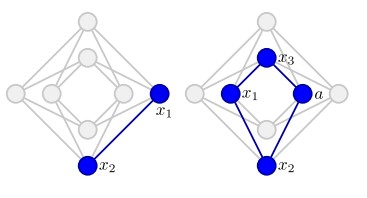
\includegraphics{Ising1+2.png}
	\caption{On the left, a valid positioning of qubits into a Chimera tile for the formula $\varphi = x_1 \iff x_2$. On the right, a valid positioning for the formula $\varphi ' = x_3 \iff (x_1 \vee x_2)$. Both architectures are inspired by the penalty functions discussed in this paragraph.}
	\end{center}
\end{figure}

\section{Issues in Encoding for Quantum Annealers}

Converting a Boolean circuit into a QUBO formulation would apparently seem an easy task to achieve: actually the nature and the architecture of the annealers drastically reduce the number of SAT problems we can embed. The main issues causing the inefficiency are:

\begin{itemize}
    \item \textbf{The number of qubits is not unlimited}: even though the recent architectures provides more than 2000 qubits, they are usually not enough to encode the majority of circuits.
    This is due by the nature of the two encoding: the number of qubits representing the input width and the circuit size are two different metrics for complexity, where the former is definitively bigger than the latter. 
    \item \textbf{The number of couplings is not unlimited}: as already mentioned in paragraph, each architecture can be interconnected to a limited number of other qubits. Consequently, the encoding process has to take into account this upper limit and, if more connections are required, map a Boolean variable into multiple qubits.
    \item 
\end{itemize}

Because of the problems described above, advanced algorithms have been studied and tested in order to reduce the amount of qubits required during the reduction.

\section{Encoding complex Boolean formulas}

Determine an efficient encoding is decisive, given the limited of number of qubits of Chimera. Penalty functions have some properties we can exploit to iteratively build complex formula from easier ones. The first property is \textbf{NPN-Equivalence}: given a boolean formula $F(\textbf{\underline{x}})$ with its associated penalty function $P_F(\underline{\textbf{x}},\underline{\textbf{a}} | \underline{\theta})$ and a new Boolean function $F^*(\textbf{\underline{x}})$ identical to the previous one but a single variable at a generic index $i$ (so that it appears with inverse cardinality in the new formulation), we can recycle $P_F(\underline{\textbf{x}},\underline{\textbf{a}} | \underline{\theta})$ to obtain the penalty function for the new problem. In particular, $P_{F^*}(\underline{\textbf{x}},\underline{\textbf{a}} | \underline{\theta}) = P_F(\underline{\textbf{x}},\underline{\textbf{a}} | \underline{\theta}^*)$ where $\theta^*$ is a new vector of biases and couplings so that for each $z,z'\in \textbf{\underline{x}},\textbf{\underline{a}}$: \\ \\ \\

\begin{equation}
    \theta_z^* = 
    \left\{
        \begin{array}{lr}
            -\theta_z, & \textit{if }z = x_i \\
            \theta_z, & otherwise
        \end{array}
    \right\}
\end{equation}

\begin{equation}
    \theta_{zz'} = 
    \left\{
        \begin{array}{lr}
            -\theta_{zz'}, & \textit{if }z = x_i \vee z' = x_i\\
            \theta_{zz'}, & otherwise
        \end{array}
    \right\}
\end{equation}


So once we extract the penalty function for a Boolean Formula, its variants can be easily computed switching signs of biases and coupling. For instance, if we had the Boolean formula $\varphi = x_1 \iff -x_2$, we could easily invert signs of couplings and biases associated with $x_2$, trivially obtaining $P_F(\underline{\textbf{x}} | \underline{\theta}) = 1 + x_1x_2$. \\
The second property fundamental to simplify the task of retrieving penalty functions is the \textbf{AND-decomposition}. Given a Boolean function that can be rewritten as a combination of simpler functions so that $F(x) = \land_k F_k(\underline{x}^k)$, where each $F_k(x)$ is associated to a penalty function $P_{F_k}(\underline{x^k},\underline{a^k}|\underline{\theta^k})$ with minimum gap $g^k_{min}$, $\underline{x} = \cup_k \underline{x^k}$ and $\underline{a} = \cup_k \underline{a^k}$, then we can define a penalty function for the original formula in the following way:

\begin{equation*}
    P_{F}(\underline{x},\underline{a}|\underline{\theta}) = \sum_k P_{F_k}(\underline{x^k},\underline{a^k}|\underline{\theta^k}) \; \textrm{        with        } g_{min} = \min_k(g^k_{min})
\end{equation*}
\begin{equation}
    \theta_i = \sum_k \theta^k_i
\end{equation}
\begin{equation*}
    \theta_{ij} = \sum_k \theta^k_{ij}
\end{equation*}

Equation 2.8 works in the case each bias and coupler value satisfies its range. The subformulas making up the decomposition could share some common variables and, in some cases, this could lead to the attainment of out-of-range biases and couplers. This issue can be easily fixed: we can scale up or down the impact of each penalty function adding a weight $w_k$ greater than 0. This addition slightly modifies equation 2.8, determining the general formulation:

\begin{equation*}
    P_{F}(\underline{x},\underline{a}|\underline{\theta}) = \sum_k P_{F_k}(\underline{x^k},\underline{a^k}|\underline{\theta^k})*w_k \; \textrm{        with        } g_{min} = \min_k(g^k_{min})*w_k
\end{equation*}
\begin{equation}
    \theta_i = \sum_k \theta^k_i*w_k
\end{equation}
\begin{equation*}
    \theta_{ij} = \sum_k \theta^k_{ij}*w_k
\end{equation*}

Adding these weights weakens the minimum gap, so it is not used in practice. An alternative to equation 2.9 relies on the renaming of the shared variable, so that each $\underline{x}^k$ is disjoint with respect to the others. To achieve this goal, when two conjuncts $F_k, F'_k$ share a Boolean variable $x_i$ we rename the second occurrence with a fresh variable $x'_i$ and conjoin the two variable using the simple formula $(x_i \iff x'_i)$. Now we can re-define the original formula and its associated penalty function as:

\begin{equation*}
    F^*(\underline{x}^*) = \bigwedge_k F_k(\underline{x}^{k*}) \land \bigwedge_{\{ x_i \textrm{  shared}\}} (x_i \iff x'_i) 
\end{equation*}
\begin{equation}
    P_{F^*}(\underline{x}^*,\underline{a}|\underline{\theta}) = \sum_k P_{F_k}(\underline{x^k},\underline{a^k}|\underline{\theta^k}) + \sum_{\{ x_i \textrm{  shared}\}} (1 - x_ix'_i)
\end{equation}
\begin{equation*}
    g_{min} = min_k(g^k_{min},2)
\end{equation*}

Given the nature of the penalty functions for $(x_i \iff x'_i)$, whose gap is 2, we ensure no issue can emerge and no parameter range error can be observed.
Combining the two properties above we can define the procedure to apply to retrieve penalty functions decomposing Boolean formulas into smaller chunks, easier to convert:

\begin{itemize}
    \item First we Tseitin-style decompose F(x) into an equi-satisfiable formula so that:
    
    \begin{equation}
        FORMULA
    \end{equation}
    \item When two conjuncts $F_1$ and $F_2$ share one variable $y_j$, rename the second with a fresh new variable $y_i'$, conjoining $(y_i' \iff y_j)$.
    \item Compute the penalty function for each conjunct separately.
    \item Sum the penalty functions obtained in the previous step to obtain a single function. 
\end{itemize}

From the algorithm described above, we can define a universal approach to deal with larger Boolean functions, avoiding the application of the SMT formulation which results too much time and resource demanding. \\
Before starting the encoding, we compute in advance a collection of valid encoding for simple SAT formulas so that they can be mapped using a low number of qubits (in particular when using the Chimera architecture we aim to encode the formula using a single tile). The original SAT formula we want to encode is pre-processed, in order to reduce its size or complexity in terms of its graphical
representation. As an example, a good pre-processing approach is using the and-inverted-graph representation, which transform a formula in a combination of AND and NOT functions. Using the simplified structure and the previously computed library we then define a mapping between Boolean variables and the annealer's qubits. This phase represents the most complex and resource-demanding procedure of the algorithm. The fundamental steps of this procedure are:

\begin{figure}[t]
	\begin{center}
	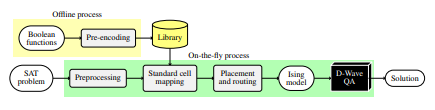
\includegraphics{LargeBool.PNG}
	\caption{A graphical representation of the encoding process for larger Boolean functions.}
	\end{center}
\end{figure}

\begin{itemize}
    \item Use the library of pre-computed penalty functions to map each function part of the decomposed and simplified SAT formula into a valid QUBO encoding. This phase is known as standard cell mapping.
    \item Now it is necessary to embed the entire formula onto the QA hardware. To achieve this task, we first assign a disjoint subgraph of the QA hardware graph to each penalty function chosen in the previous step.
    \item Lastly we need to ensure that qubits representing the same variable are chained so that they can assume the same value when given as input to the annealer: we can accomplish it using penalty functions in the form $1 - x_1x_2$, where $x_1$ and $x_2$ are qubits representing the same variable. This step is a direct consequence to formula 2.8.
\end{itemize}

The algorithm is heavily discussed in \cite{varotti} and more details are provided about the choice of and the heuristic adopted to obtain a more stable encoding, but for the sake of brevity we will not discuss it further. Figure 2.4 summarizes the entire process.

\pagebreak

